%%%%%%%%%%%%%%%%%%%%%%%%%%%%%%%%%%%%%%%%%%%%%%%%%%%%%%%%%%%%%%%%%%%%%%%%
%    INSTITUTE OF PHYSICS PUBLISHING                                   %
%                                                                      %
%   `Preparing an article for publication in an Institute of Physics   %
%    Publishing journal using LaTeX'                                   %
%                                                                      %
%    LaTeX source code `ioplau2e.tex' used to generate `author         %
%    guidelines', the documentation explaining and demonstrating use   %
%    of the Institute of Physics Publishing LaTeX preprint files       %
%    `iopart.cls, iopart12.clo and iopart10.clo'.                      %
%                                                                      %
%    `ioplau2e.tex' itself uses LaTeX with `iopart.cls'                %
%                                                                      %
%%%%%%%%%%%%%%%%%%%%%%%%%%%%%%%%%%
%
%
% First we have a character check
%
% ! exclamation mark    " double quote
% # hash                ` opening quote (grave)
% & ampersand           ' closing quote (acute)
% $ dollar              % percent
% ( open parenthesis    ) close paren.
% - hyphen              = equals sign
% | vertical bar        ~ tilde
% @ at sign             _ underscore
% { open curly brace    } close curly
% [ open square         ] close square bracket
% + plus sign           ; semi-colon
% * asterisk            : colon
% < open angle bracket  > close angle
% , comma               . full stop
% ? question mark       / forward slash
% \ backslash           ^ circumflex
%
% ABCDEFGHIJKLMNOPQRSTUVWXYZ
% abcdefghijklmnopqrstuvwxyz
% 1234567890
%
%%%%%%%%%%%%%%%%%%%%%%%%%%%%%%%%%%%%%%%%%%%%%%%%%%%%%%%%%%%%%%%%%%%
%
\documentclass[10pt]{iopart}
%\documentclass[12pt]{iopart}
%\newcommand{\gguide}{{\it Preparing graphics for IOP Publishing journals}}
%Uncomment next line if AMS fonts required
%\usepackage{iopams}
\usepackage{graphicx}
\usepackage{multirow}
\usepackage{amssymb}
\usepackage{url}
\begin{document}

\title[Computer vision for quantifying Fe-related defects in Si solar cell]{Computer vision-based method for quantifying iron-related defects in silicon solar cell}

\author{Oleg Olikh\footnote{Author to whom any correspondence should be addressed.}, Oleksii Zavhorodnii, Yulia Perets}

\address{Taras Shevchenko National University of Kyiv, Kyiv 01601, Ukraine}

\ead{olegolikh@knu.ua}
%\vspace{10pt}
%\begin{indented}
%\item[]August 2017
%\end{indented}

\begin{abstract}
abstract abstract abstract abstract abstract abstract
\end{abstract}

%
% Uncomment for keywords
\vspace{2pc}
\noindent{\it Keywords}: defect, Si solar cell, iron contamination, machine learning, computer vision

% Uncomment for Submitted to journal title message
\submitto{\SST}
%
% Uncomment if a separate title page is required
%\maketitle

% For two-column output uncomment the next line and choose [10pt] rather than [12pt] in the \documentclass declaration
\ioptwocol
%


\section{Introduction}\label{sec:Int}

Due to the urgent need to address environmental challenges and the growing global demand for renewable energy, the deployment of photovoltaic (PV) systems has been rapidly increasing worldwide.
In particular, solar PV generation exceeded 1,600 TWh in 2023 \cite{IEA2024Renewables, OSAMA2025}, rose by about 30\% in 2024 \cite{Prometheus2025}, and forecasts indicate that total installed capacity will surpass 6 TW by 2030 \cite{IEA2024Renewables}.
Meanwhile, crystalline silicon photovoltaics, which have benefited from decades of scientific advancement and continuous cost reductions, continued to dominate the market in 2024, accounting for approximately 98\% of the global share \cite{Fischer2025ITRPV, THOME2025}.

As in other semiconductor devices, defects play a decisive role in determining the operating parameters of solar cells.
Therefore, diagnosing defects, particularly determining their concentrations, is critically important for maintaining the stable performance of PV systems.
In recent years, researchers have increasingly complemented established defect-characterisation methods with machine learning (ML) approaches that improve the accuracy, speed, and cost efficiency of these analyses.
The use of ML methods for analysing macroscopic defects (such as cracks, finger failures, hotspots, and scratches) and point defects, however, differs significantly.
Researchers typically detect macroscopic defects in PV systems using two main approaches \cite{Jia2024, Hijjawi2023}.
The first approach, Electrical Testing Techniques, involves analysing characteristic electrical curves of parameters such as current, voltage, and power.
The second approach, Imaging-Based Techniques, involves analysing electroluminescence (EL) \cite{Liu2024a} or photoluminescence \cite{Doll2021} images of solar cells.
Numerous review studies demonstrate extensive use of ML in both approaches \cite{Datta2023, Jaiswal2023, Buratti2024, MAHDAVIPOUR, Hopwood2020, Li2021, Liu2021}.

Regarding point defects, although they represent one of the primary limitations of PV devices, researchers have developed considerably fewer ML techniques specifically for their analysis.
Existing ML-based approaches include extracting recombination-active centre parameters from lifetime measurements \cite{Wang2024a, Buratti2022, Buratti2020a},
detecting radiation-induced defects using Raman spectroscopy \cite{Park2022, Chia2024}, 
estimating the concentration of contaminant impurities from the ideality factor of current–voltage characteristics \cite{Olikh2022PPV}, 
and analysing variations in photovoltaic conversion parameters \cite{Olikh2025SE}.
Nevertheless, a relatively limited number of such methods are offered.


One of the main challenges in applying ML methods effectively is that training the models requires a large amount of labelled data \cite{Buratti2024}.
In practice, researchers often cannot obtain such large volumes of experimental data; 
therefore, they commonly employ approaches such as simulations, 
in which hundreds of thousands of dependencies are computed \cite{Wang2024a, Buratti2022, Buratti2020a, Olikh2025MSEB, Olikh2025SE}; 
Physics-Informed Neural Networks (PINNs), which incorporate physical laws into the loss function to generate synthetic data \cite{Wang2024b, Li2025}; 
or Transfer Learning, in which a model trained on one task is adapted to another related task \cite{Kaya2019, Kim2023}.
However, simulations can be highly demanding in terms of time and computational resources; PINNs are primarily suitable for phenomena described by partial differential equations, and pre-trained models are not available for all types of physical problems.
At the same time, one of the most extensively studied tasks in machine learning is computer vision (CV), 
for which many pre-trained models have been publicly released. 
Moreover, these models are typically trained on extremely large standard datasets. 
For example, EfficientNetB7 was trained on approximately 1.2 million images from the ImageNet dataset.

This work primarily aimed to apply standard pre-trained CV models to analyse electrophysical measurement results related to point defects.
In particular, we focused on quantifying iron in boron-doped crystalline silicon solar cells by examining the short-circuit current 
($I_\mathtt{SC}$) relaxation following intense illumination.
Iron represents one of the most prevalent, ubiquitous, and efficiency-limiting metallic impurities in such structures \cite{Buonassisi2006, IronSC}, 
which, as noted earlier, form the foundation of the photovoltaic market.
In Si:B, iron tends to form iron–boron pairs under equilibrium conditions, which intense illumination can dissociate \cite{Kimerling1983, FeBAssJAP2014}.
In fact, the aforementioned $I_\mathtt{SC}$ variations directly reflect the recovery process of iron–boron pairs \cite{Olikh2021JAP}.


It should be noted that the use of well-established computer vision benchmark architectures such 
as YOLO, MobileNetV2, EfficientNet, ResNet, Xception, GoogleNet, and other convolutional neural networks (CNNs) is a common approach for identifying macrodefects from EL
measurements \cite{Liu2024a, Li2024a, Jia2024, Otamendi2021, Chen2022, AlOtum2024, Abdelsattar2025, tella2025}. 
However, in this case, the measurement result is an image, which makes the approach relatively straightforward.
In our case, it was necessary to transform the time dependence into an image representation.
Standard approaches to solving such problems involve the use of Fourier or wavelet transforms, and last were applied in this study.
In photovoltaics, wavelet transforms are typically used for processing solar cell images to enhance the detection of
macrodefects \cite{Li2012, Rosa2024}, but they can also be employed to convert one-dimensional non-stationary signals into two-dimensional spectrograms and thereby enable the effective extraction of subtle features \cite{Vinit2020}.

By applying computer vision models to wavelet spectrograms represented as images, we generated high-dimensional feature vectors and used them as inputs for traditional regression models.
The $I_\mathtt{SC}$(t) dependencies for training the regression models were obtained through both simulation and experimental measurements.
In both cases, the hybrid Transfer Learning approach produced predictions with sufficiently high accuracy (within a few percent), even when training models on small datasets containing fewer than 30 samples.
Importantly, the proposed approach is highly versatile and can be extended to a wide range of tasks related to defect characterization and other applications.


\section{Methodology}\label{sec:Exp}

\subsection{General outline of the method}\label{subsec:GenSch}

\Fref{Fig1} illustrates the workflow of the ML pipeline used to extract iron contamination from $I_\mathtt{SC}(t)$ dependencies.
The process consists of three main blocks: Data Acquisition, CNN Feature Processing, and Predictive Regression.
The first stage involves either simulating or experimentally measuring the time dependence 
of the short-circuit current in a solar cell after the induced decay of FeB pairs. 
These procedures are described in more detail in Subsections~\ref{subsec:SimDet} and \ref{subsec:ExpDet}.
For the experimental curves, the data were smoothed using a Savitzky–Golay filter \cite{Krishnan2013}. 
Subsequently, a continuous wavelet transform \cite{Torrence1998} was applied to convert the one-dimensional time dependencies 
into two-dimensional spectrograms represented as images, 
where each point corresponds to the amplitude of the wavelet coefficient at a specific time and frequency. 
The Morlet wavelet was employed, and the procedure was implemented using the Python package PyWavelets. 
Examples of the resulting images are shown in \Fref{Fig2}b and \Fref{Fig2}c. 
Data augmentation was then performed by flipping the images along the x- and y-axes and rotating them by 90$^{\circ}$, 180$^{\circ}$, and 270$^{\circ}$.
This procedure is known to improve the accuracy of ML model predictions, particularly when only small datasets are available \cite{Ahmad2020}.


\begin{figure*}
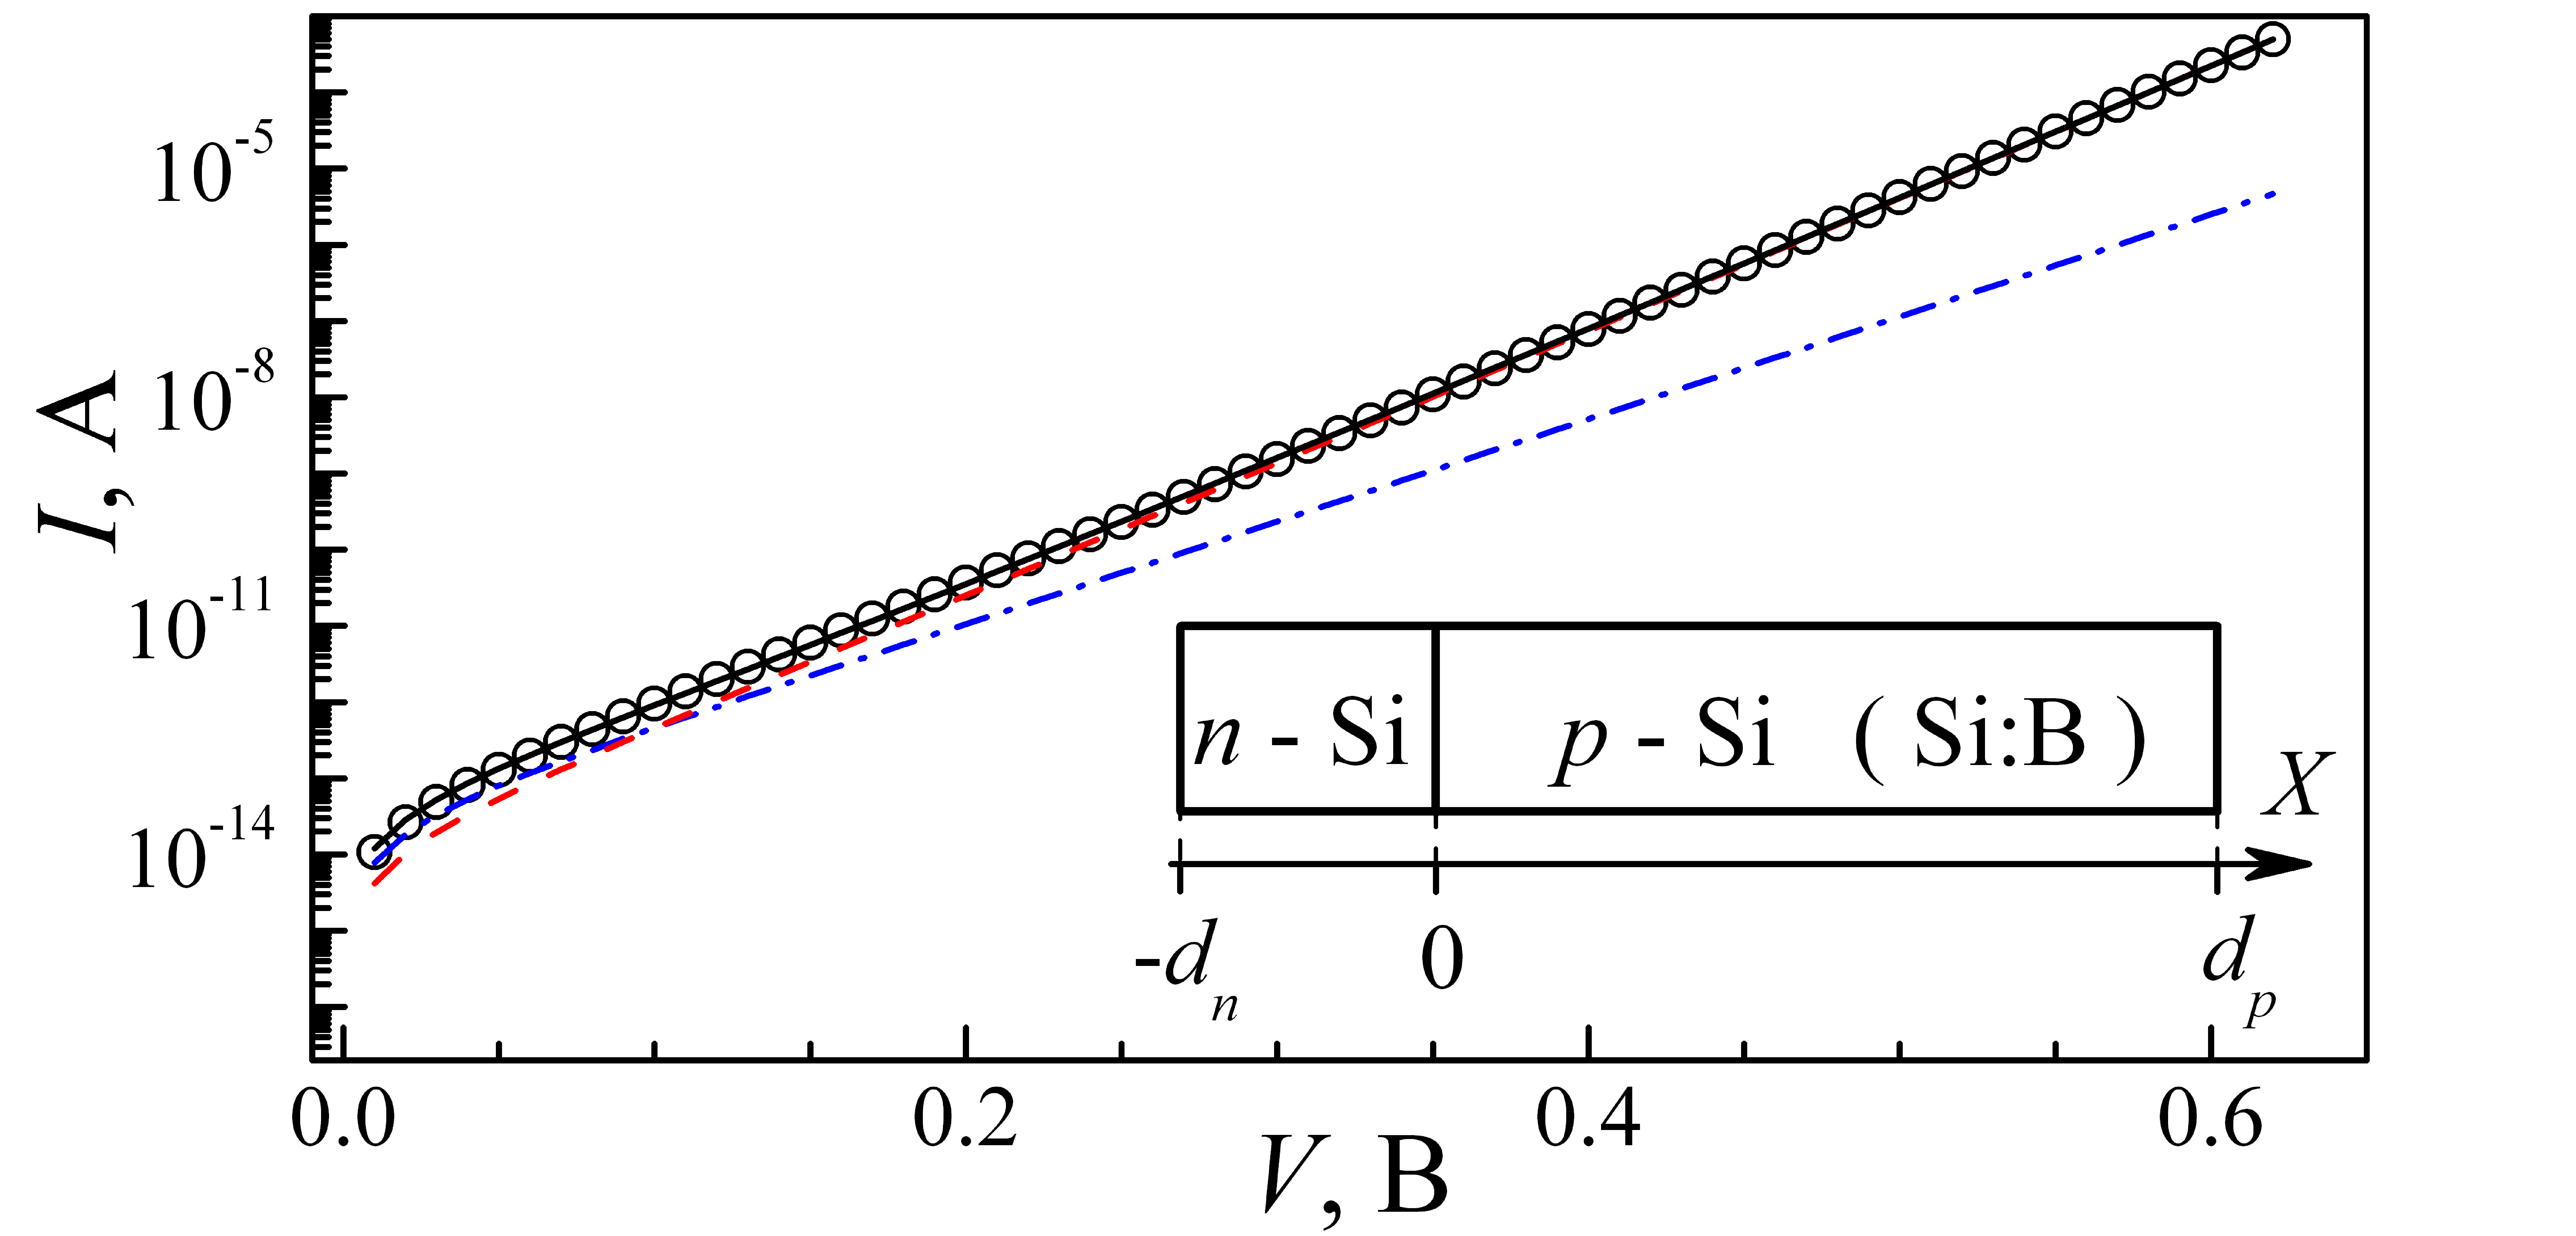
\includegraphics[width=0.95\textwidth]{Fig1}
\caption{\label{Fig1}
The workflow of the ML pipeline
}%
\end{figure*}

\begin{figure}
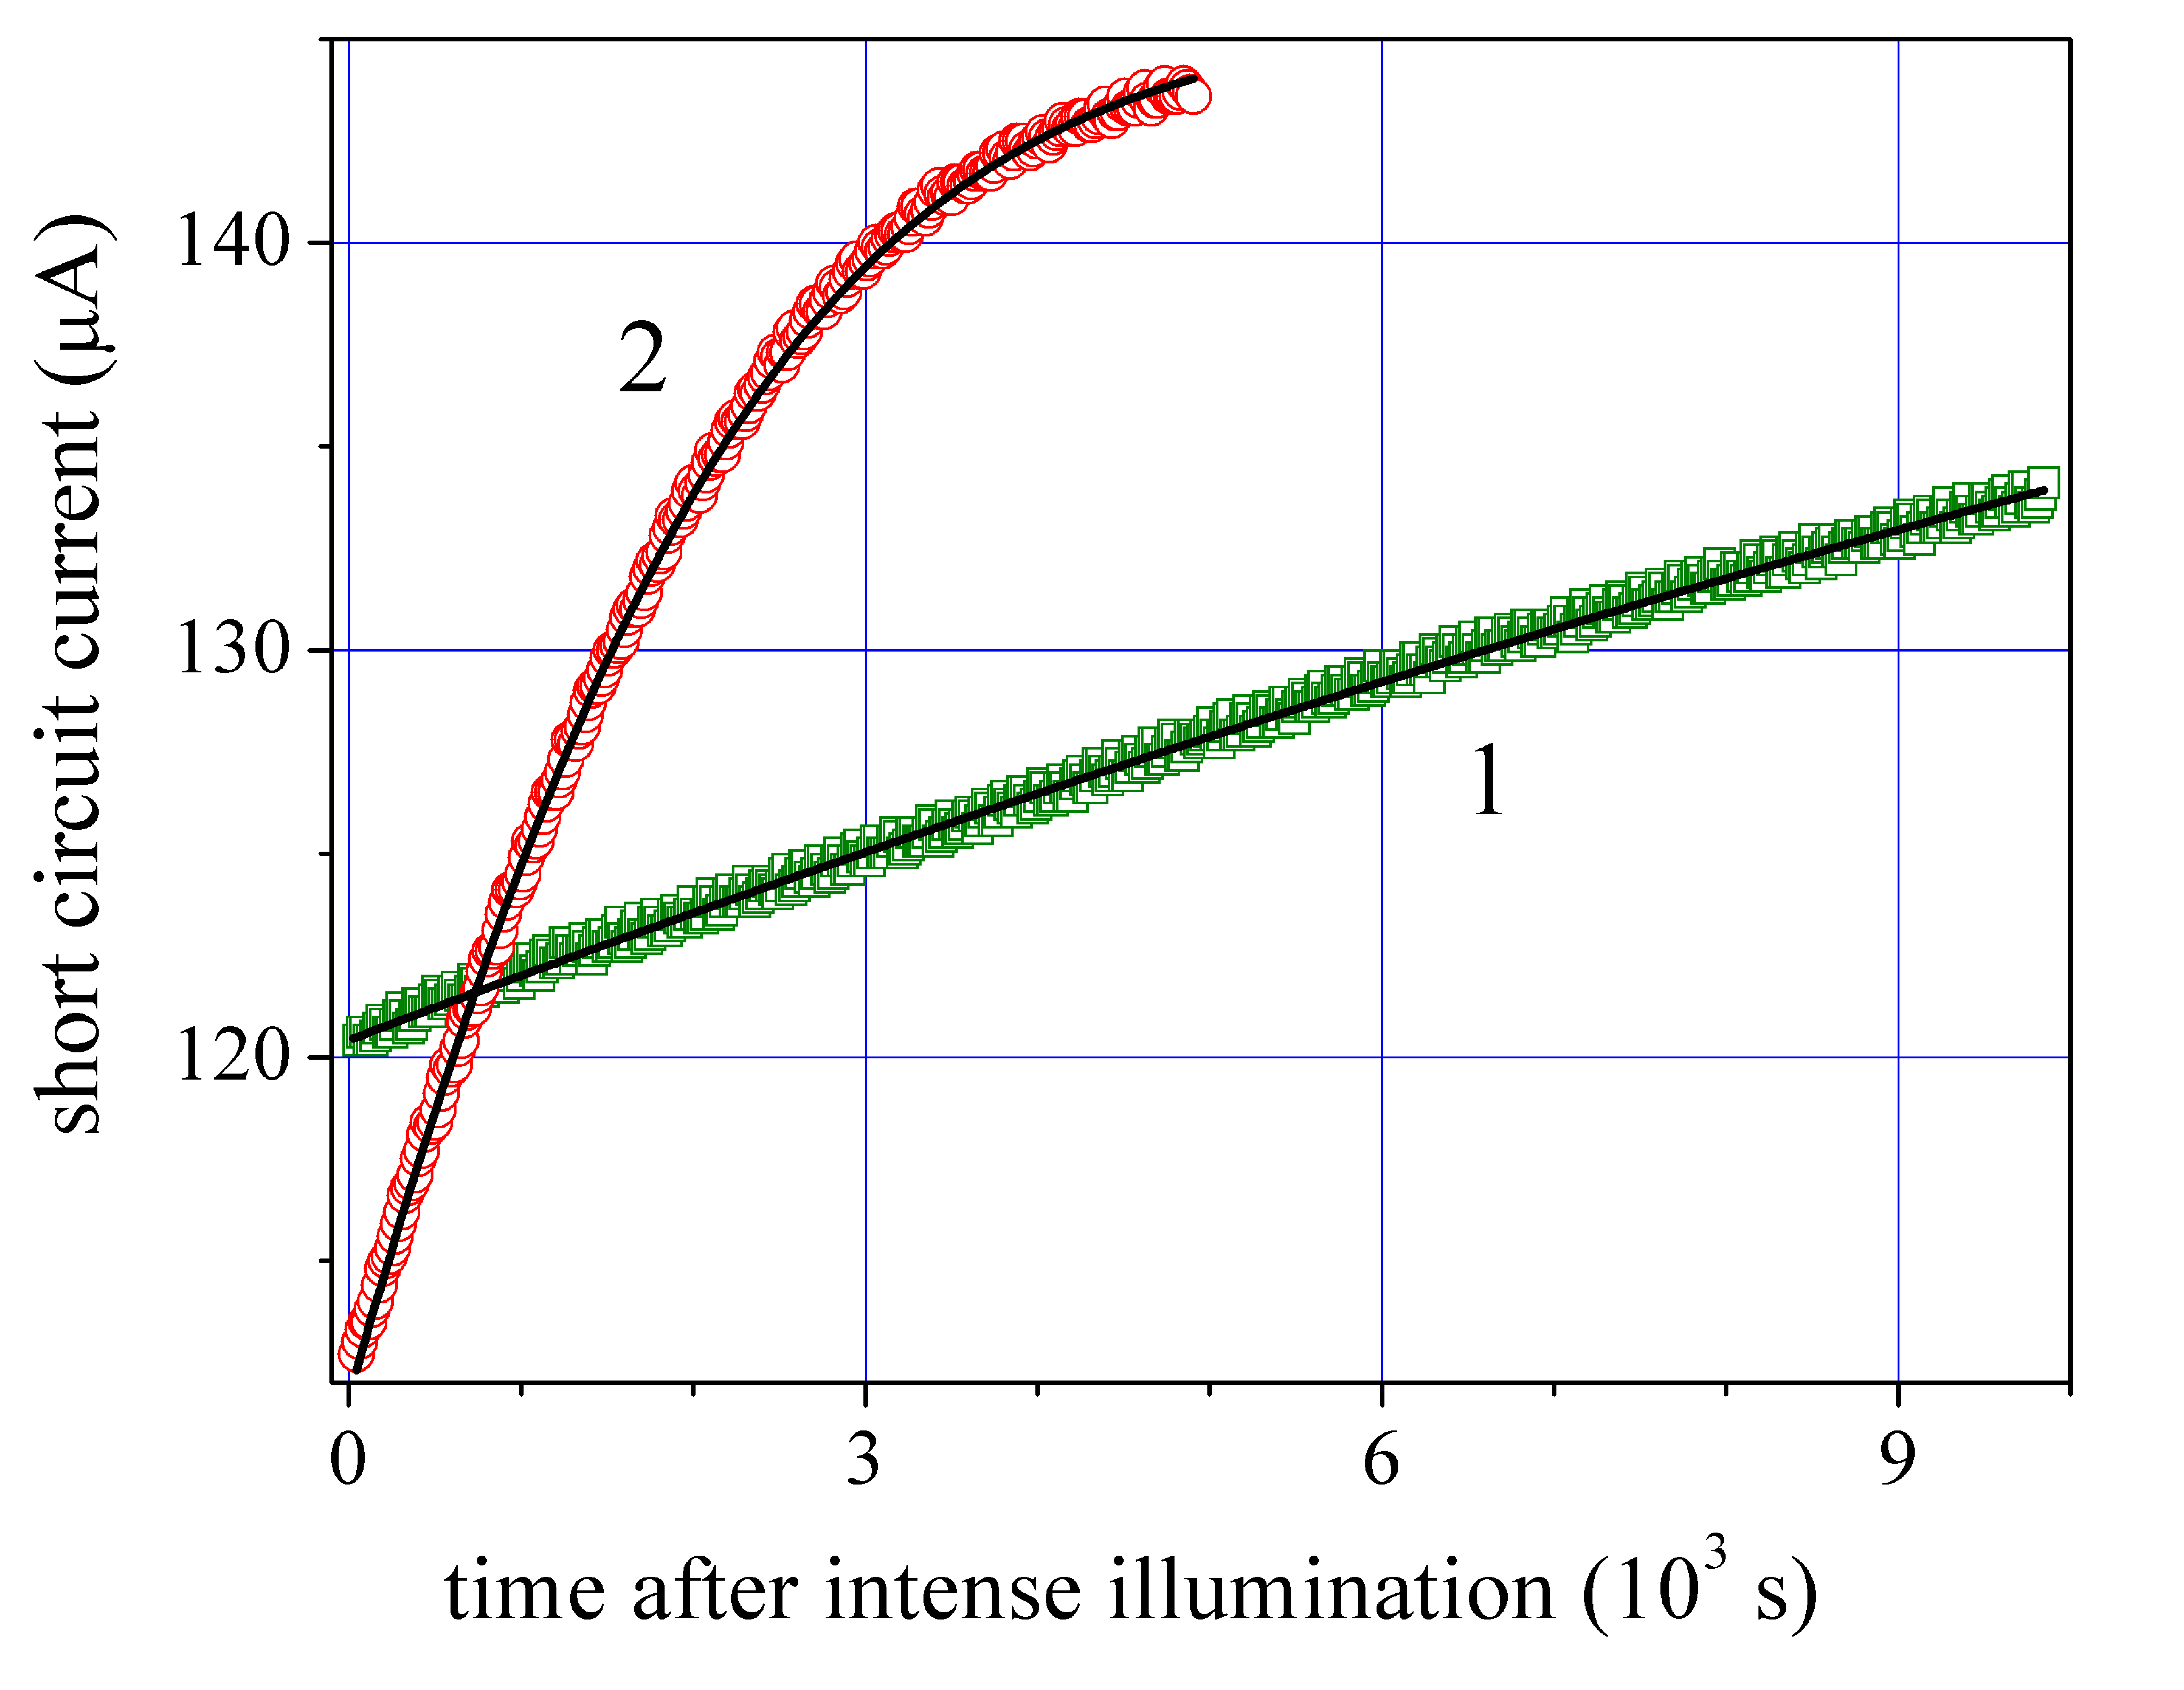
\includegraphics[width=0.5\textwidth]{Fig2}
\caption{\label{Fig2}
Simulated time dependencies of the short-circuit current (a) 
and the corresponding wavelet spectrograms for iron concentrations 
of $10^{10}$~cm$^{-3}$ (b) and $10^{14}$~cm$^{-3}$ (c).
The data in panel a are shown with filled squares for the concentration corresponding to panel b
and with open circles for that corresponding to panel c.
}%
\end{figure}


During the CNN Feature Processing stage, all images (both original and augmented) were processed using one of the standard CV models 
to extract a feature set for each image. 
The selected models and feature extraction settings are described in Subsection~\ref{subsec:CompVisMod}. 
No CNN fine-tuning was performed; the models were used in their pre-trained form as downloaded.
In general, the dimensionality of the feature vectors obtained from CNN outputs substantially exceeds the number of available samples, 
implying a high degree of redundancy. 
Therefore, to enable comparison and mitigate this effect, Principal Component Analysis (PCA) was applied in some cases 
to reduce the feature dimensionality with negligible loss of total variance.


The obtained feature sets served as inputs to regression models based on one of the standard algorithms described in Subsection~\ref{subsec:RegAlg}, 
which aimed to predict the iron concentration ($N_\mathtt{Fe}$) in the solar cell.
%The regression models were trained on a training dataset and validated on a test dataset using the evaluation metrics outlined in Subsection~\ref{subsec:ModEva}.
%During training, we treated the feature sets corresponding to the original wavelet spectrogram and the augmented images as individual samples. During testing, we obtained the final prediction by taking the median value from the outputs corresponding to the augmented images.
%In one case, we trained the models on simulated data and tested them on both simulated and experimental datasets. In another, we used part of the experimental data for training and the remaining portion for testing.

In the first case, the regression models were trained on a simulated training dataset and tested on both the simulated test dataset and experimental data.
In the second case, a portion of the experimental results was used for training, while the remaining part was reserved for testing the corresponding models.
During training, feature sets derived from the original wavelet spectrograms and their augmented versions were treated as separate samples.
During testing, the median of the predicted values obtained from the original and augmented images was used as the final prediction.
Model performance was evaluated using the metrics described in Subsection~\ref{subsec:ModEva}.




\subsection{Simulation details}\label{subsec:SimDet}
%
%This study performed I–V curve simulations for a silicon $n^+$-$p$-$p^+$ structure under monochromatic illumination using SCAPS 3.3.11 to obtain the $I_\mathtt{SC}$(t) dependencies.
%The SCAPS-1D software \cite{SCAPS1} serves as a widely used tool for modelling solar cells with defect-state effects \cite{MasumMia2025, Joshi2024, Ravidas2024, Liu2024, You2023, SCAPSDefect3}.
%The study extracted $I_\mathtt{SC}$ values from the simulated I–V curves following a standard procedure \cite{SCparam2017}.
%
%
%During the simulations, we assumed that the base thickness of the structure was 380~$\mu$m, that the dopant was boron with a concentration of $N_\mathrm{B} = 1.36 \times 10^{15}$ cm$^{-3}$, and that the temperature was 340~K.
%We provided illumination using light with a wavelength of 940~nm and an intensity of 5 W/m$^{2}$, matching the experimental conditions (see \ref{ExpDet}).
%We set the total concentration of iron impurity atoms, $N_\mathtt{Fe}$, as one of the simulation parameters.
%We assumed that the atoms were uniformly distributed throughout the base and $p^+$ layer of the solar cell and could exist either in the interstitial position (concentration $N_\mathtt{Fe_i}$) or as iron–boron pairs (concentration $N_\mathtt{FeB}$).
%The time dependence of $N_\mathtt{Fe_i}$ after pair dissociation follows the well-known expression \cite{MurphyJAP2011, Wijaranakula}:
%
%\begin{equation}\label{eqNFet}
%  N_\mathtt{Fe}(t)=(N_\mathtt{Fe_i,0}-N_\mathtt{Fe,eq}) \times \mathtt{exp}({-t/\tau_{ass}})+N_\mathtt{Fe,eq},
%\end{equation}
%
%\begin{equation}\label{eqtauass}
%  \tau_{ass}=5.7 \times 10^5 \frac{\mathrm{s}}{\mathrm{Kcm^{-3}}} \times \frac{T}{N_\mathtt{A}}\mathtt{exp}(\frac{E_\mathtt{m}}{kT}),
%\end{equation}
%
%where $\tau_{ass}$ is the characteristic of the  complex association, $N_\mathtt{Fe_i,0}$ is the concentration of interstitial iron atoms formed due to FeB pair dissosiation, $N_\mathtt{Fe_i,0}$ = $N_\mathtt{Fe_i}$(t=0) = $N_\mathtt{Fe}$, and $N_\mathtt{Fe,eq}$ is the portion of interstitial iron atoms that remain unpaired in the equilibrium state $N_\mathtt{Fe,eq}=N_\mathtt{Fe_i}$(t $\rightarrow \infty$).
%According to \cite{MurphyJAP2011, Wijaranakula}
%
%\begin{equation}\label{eqFeieq}
%  [Fe_{i,\mathtt{eq}}]=\frac{Fe_{\mathtt{bulk}}}{[1+N_\mathtt{A}10^{-23}\mathtt{exp}(\frac{E_\mathtt{b}}{kT})][1+\mathtt{exp}(\frac{E_\mathtt{F}-0.39eV}{kT})]},
%\end{equation}
%
%where $E_\mathtt{b}$ is the binding energy of the FeB pairs and $F$ is the Fermi level (donor level $E_\mathtt{Fe_i}=E_V+0.394~eV$ is associated with Fe$_i$).
%
%
%In turn, the study estimated the iron–boron pair concentration $N_\mathtt{FeB}$ from
%
%\begin{equation}\label{eqNFeB}
%  N_\mathtt{FeB}(t)+N_\mathtt{Fe}(t)=N_\mathtt{Fe,0},
%\end{equation}
%
%Overall, the concentrations of iron-related defects depended not only on time but also on their spatial position within the structure, reflecting the non-uniformity of the $F$–$E_\mathtt{Fe_i}$ difference.
%Olikh et al. \cite{Olikh2025MSEB, Olikh2019SM} provide a detailed description of the modelling approach, including the values of silicon and defect parameters.
%To create the training dataset, we used 25 $N_\mathtt{Fe}$ values, uniformly distributed on a logarithmic scale from $10^{10}$~cm$^{-3}$ to $10^{14}$~cm$^{-3}$.
%\Fref{Figure 2} shows examples of the resulting $I_\mathtt{SC}$(t) dependencies and the corresponding wavelet spectrograms.
%We generated the simulated test dataset using 10 $N_\mathtt{Fe}$ values not included in the training set.

\subsection{Experiment details}\label{subsec:ExpDet}

%We validated the proposed method using measurements of $n^+$-$p$-$p^+$ silicon solar cells fabricated on 380~$\mu$m thick $p$-type boron-doped Cz-wafers ($N_\mathrm{B}=1.36\times10^{15}$~cm$^{-3}$).
%The $n^+$ (0.7~$\mu$m, 20–30 $\Omega$/$\Box$) and $p^+$ (0.6~$\mu$m, 10–20 $\Omega$/$\Box$) layers were formed by phosphorus and boron diffusion, respectively; details of the fabrication are given elsewhere \cite{Olikh2021JAP}.
%Current–voltage curves and $I_\mathtt{SC}$ kinetics were measured with a Keithley 2450 source meter. A 940~nm SN-HPIR940nm-1W LED ( intensity 5 W/m$^{2}$) served as a low-intensity monochromatic source, with its output stabilized by a W1209 thermostat and a feedback-controlled power supply.
%The cell temperature was regulated by a thermoelectric cooler with an STS-21 sensor and maintained constant by a PID algorithm in the control software.
%FeB-pair dissociation was induced by intense (about 7000 W/m$^{2}$) halogen-lamp illumination.
%The illumination intervals were selected according to a previous study \cite{OlikhPSSA}.
%We measured the kinetics of the short-circuit current in the dark at 340~K over a period of 3000~s.
%According to Eq.~\eref{2}, this interval is sufficient for the pairs to recover fully to their equilibrium concentration.
%
%
%\Fref{Figure 3a} presents an example of a measured $I_\mathtt{SC}$(t) dependence.
%The signal contains some noise because, despite using a thermostat, the LED temperature fluctuated by approximately 0.4~K.
%We smoothed the data using a Savitzky–Golay filter, adaptively selecting the window length and filter order according to Krishnan and Seelamantula \cite{Krishnan2013}.
%For the wavelet transform, we used only the current values at the same time points as in the simulations.
%\Fref{Figure 3a} shows the corresponding smoothed curve, while the other panels display the spectrograms derived from the raw experimental curve and the processed dependence.
%
\begin{figure}
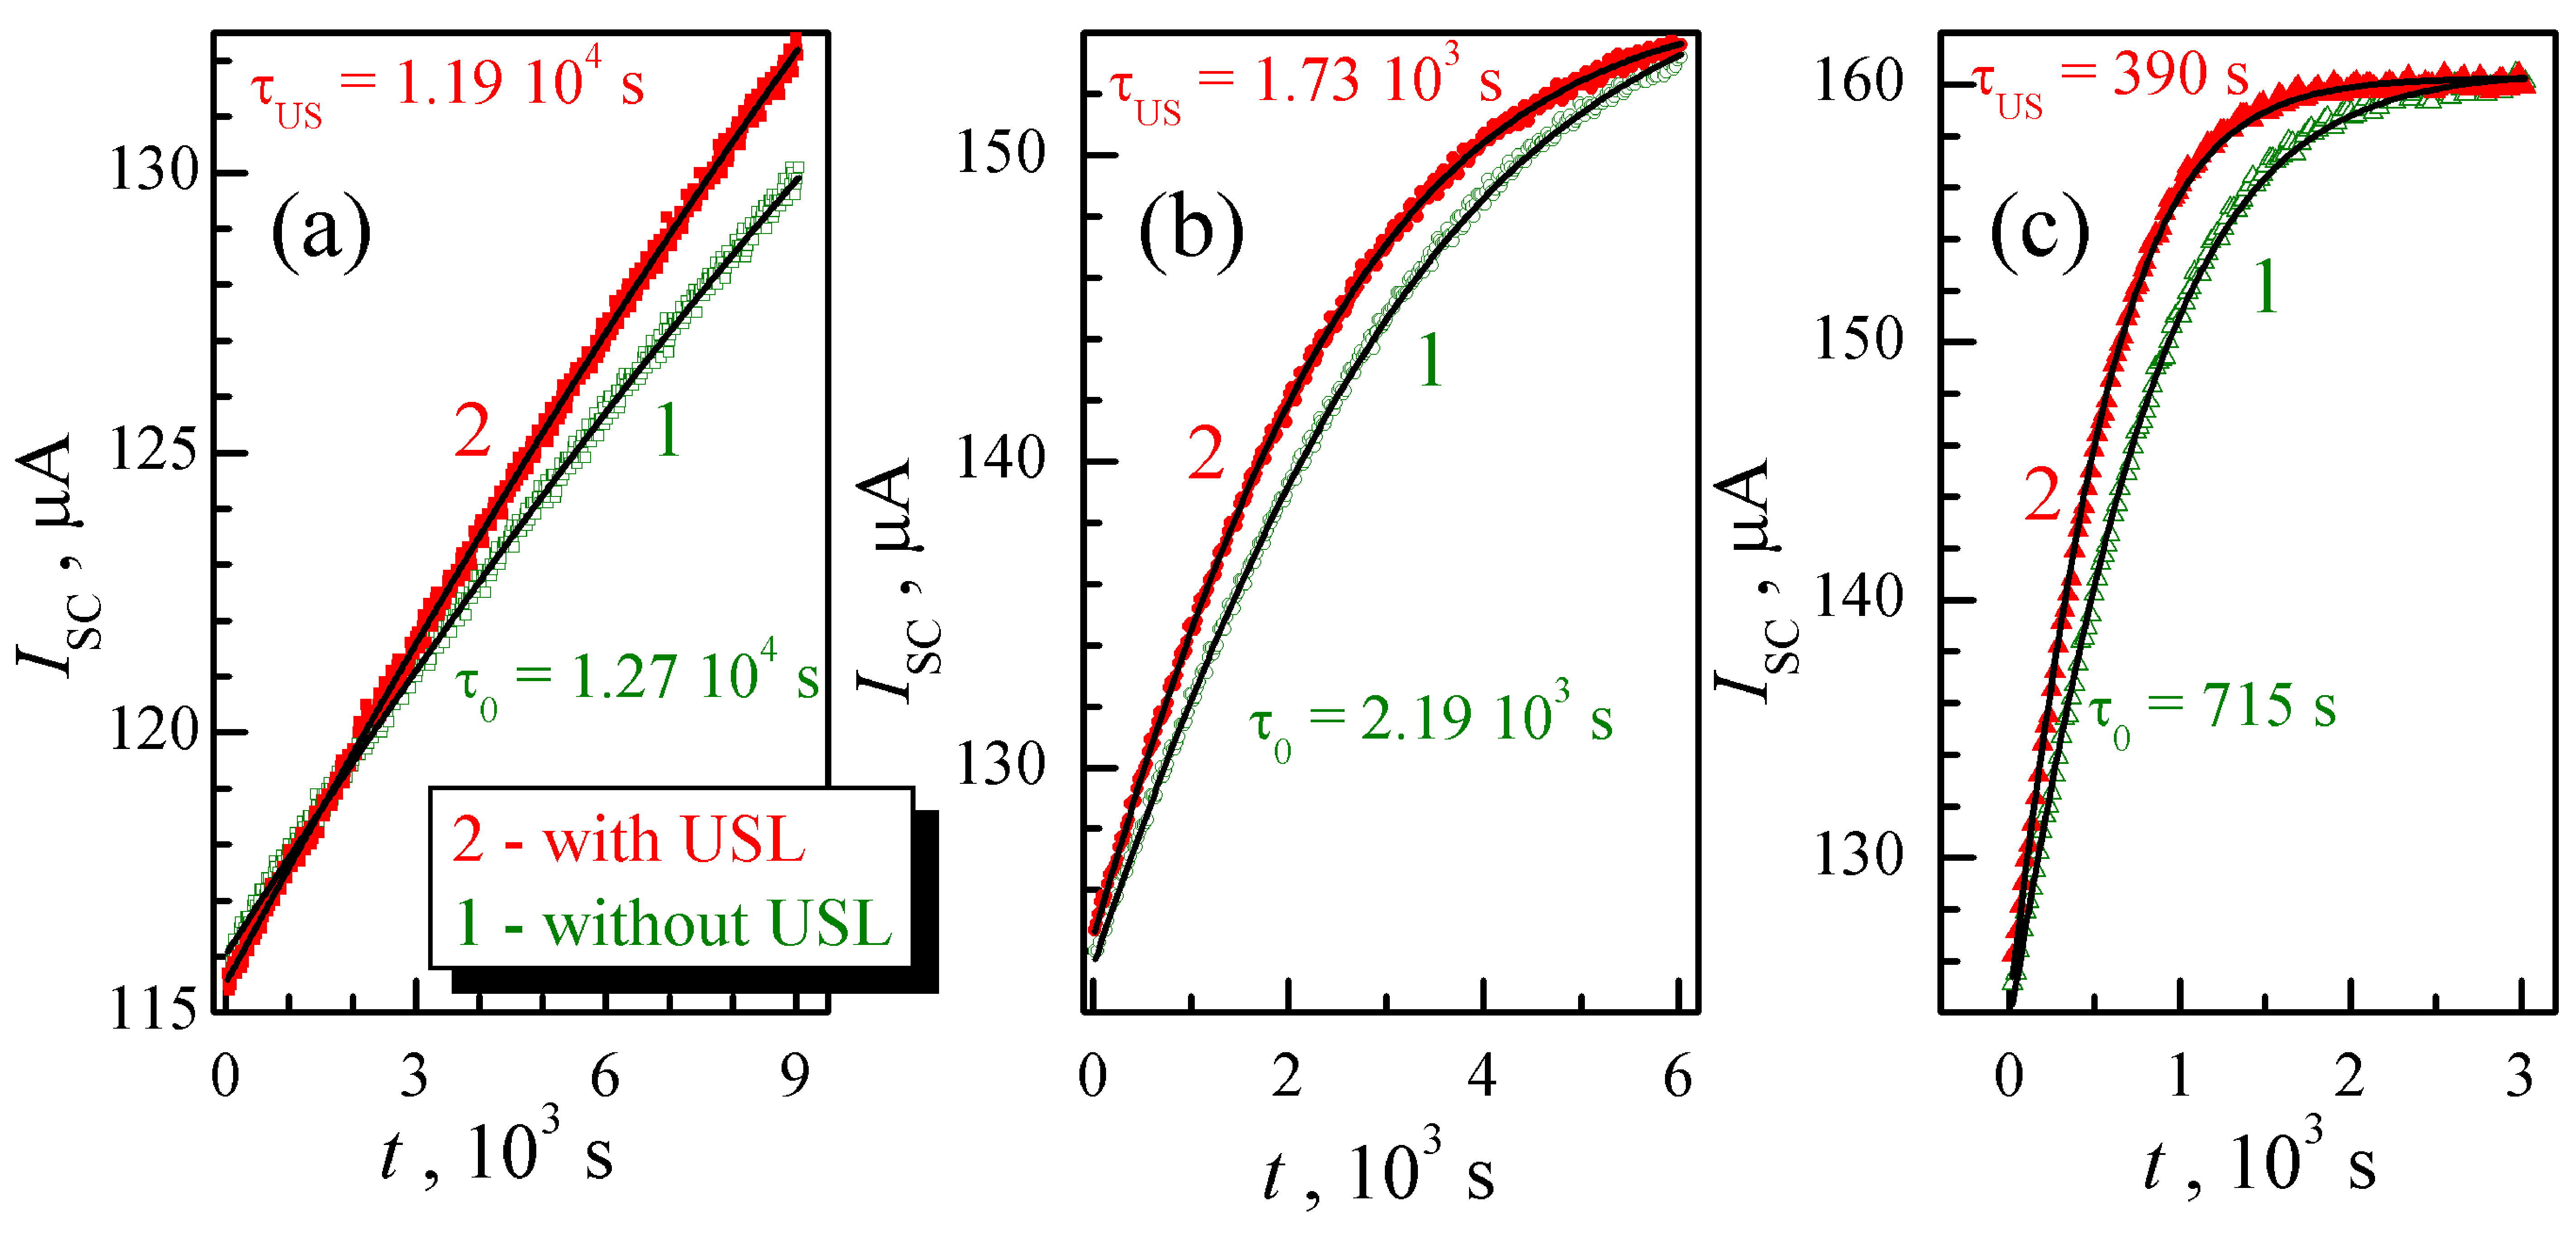
\includegraphics[width=0.5\textwidth]{Fig3}
\caption{\label{Fig3}
(a) Experimentally measured time dependence of the short-circuit current for a sample with
$N_\mathtt{Fe}=2.8\cdot10^{13}$~cm$^{-3}$ (a, filled squares) and the same dependence after applying the Savitzky–Golay filter (open circles).
Panels (b) and (c) show the wavelet spectrograms corresponding to the curves with filled squares and open circles, respectively.
}%
\end{figure}

%
%The iron concentration $N_\mathtt{Fe}$ was determined using a methodology described in \cite{Olikh2022:JMatSci,Olikh2021JAP}, which is based on fitting the kinetics of the short circuit current following FeB pairs dissociation.
%We analysed 28 samples with iron concentrations ranging from $10^{11}$~cm$^{-3}$ to $2\times10^{13}$~cm$^{-3}$.
%To test models trained on simulated data, we used all experimental measurements.
%For models trained on experimental results, we randomly selected 28 samples for training and assigned the remaining 8 samples to the test set.

\subsection{Computer vision models}\label{subsec:CompVisMod}

%To extract graphical features from the wavelet spectrograms, we applied several computer vision models available in Keras, namely EfficientNetB7, ResNet152V2, MobileNetV2, Xception, and NASNetLarge.
%All these models belong to the class of convolutional neural networks (CNNs) designed for object classification, and researchers have successfully applied them to process EL images of solar cells \cite{Jia2024, Otamendi2021, Chen2022, Abdelsattar2025, tella2025}.
%For each model, we employed two feature extraction approaches: we either passed the class probabilities, indicating the likelihood of the image belonging to a specific class, to the next stage of the pipeline, or we used the features directly extracted by the CNN.
%
%
%We also applied the CSPDarknet53 model, which serves as the CNN backbone for YOLOv4.
%This family of models features a more complex CNN architecture, optimised for detecting multiple objects in an image rather than single-object classification.
%Researchers widely use these models in Imaging-Based Techniques \cite{Liu2024a, Li2024a, Chen2022}.
%CSPDarknet53 returns three feature layers, and we processed either only the highest-level layer or the last two layers, depending on the analysis.
%
%
%Increasing the feature dimension does not constantly improve the total information variance.
%To reduce the impact of redundant data, we applied PCA, which constructs new, uncorrelated features (principal components).
%PCA is a widely used and effective tool in machine learning, particularly for improving results in Electrical Testing Techniques \cite{Fadhel2019, Gao2020}.
%We applied PCA to the training datasets using an explained variance threshold of 99.9\%, retaining only the principal components that together account for at least 99.9\% of the total variance of the original features.
%This procedure significantly reduced the feature dimensionality.
%We applied PCA only to the computer vision models that performed best on the test datasets without PCA, in order to assess the usefulness of this preprocessing step.
%Because YOLOv4 extracts a vast number of features, we also applied an additional dimensionality reduction technique.
%Specifically, we performed global average pooling on each convolutional feature map, replacing the spatial map with its mean value and thus producing one scalar per channel.
%We summarise the computer vision model variants in \tref{tabUsedMod}, along with the notations used in the subsequent analysis.
%
%\begin{table*}[]
%\centering
%\caption{Summary of used pretrained CNN models and feature extraction variants \label{tabUsedMod}}
%\begin{indented}
%\item[]
%\begin{tabular}{|c|c|c|c|c|}
%\hline
%Base model &
%  Model type &
%  Feature processing &
%  Output dimension &
%  Model Label \\ \hline
%EfficientNetB7 & Classifier        & None & 1000 & ENB7:CL   \\ \hline
%               & Feature extractor & None & 2560 & ENB7:FE   \\ \hline
%               &                   & PCA  & 39   & ENB7:FE:P \\ \hline
%MobileNetV2    & Classifier        & None & 1000 & MNV2:CL   \\ \hline
%               & Feature extractor & None & 1280 & MNV2:FE   \\ \hline
%               &                   & PCA  & 124  & MNV2:FE:P \\ \hline
%NASNetLarge    & Classifier        & None & 1000 & NAS:CL    \\ \hline
%               &                   & PCA  & 30   & NAS:CL:P  \\ \hline
%               & Feature extractor & None & 4032 & NAS:FE    \\ \hline
%ResNet152V2    & Classifier        & None & 1000 & R152:CL   \\ \hline
%               & Feature extractor & None & 2048 & R152:FE   \\ \hline
%Xception       & Classifier        & None & 1000 & XCP:CL    \\ \hline
%               & Feature extractor & None & 2048 & XCP:FE    \\ \hline
%\begin{tabular}[c]{@{}c@{}}YOLOv4 \\ (CSPDarknet53)\end{tabular} &
%  \begin{tabular}[c]{@{}c@{}}Feature extractor \\ (raw, top layer)\end{tabular} &
%  None &
%  86528 &
%  YL:FE1 \\ \hline
%               &                   & PCA  & 137  & YL:FE1:P  \\ \hline
%\begin{tabular}[c]{@{}c@{}}CSPDarknet53 \\ (YOLO backbone)\end{tabular} &
%  \begin{tabular}[c]{@{}c@{}}Feature extractor \\ (raw, top \& penultimate layers)\end{tabular} &
%  None &
%  433640 &
%  YL:FE2 \\ \hline
%               &                   & PCA  & 142  & YL:FE2:P  \\ \hline
% &
%  \begin{tabular}[c]{@{}c@{}}Feature extractor \\ (pooled, top layer)\end{tabular} &
%  None &
%  512 &
%  YL:FP1 \\ \hline
% &
%  \begin{tabular}[c]{@{}c@{}}Feature extractor \\ (pooled, top \& penultimate layers)\end{tabular} &
%  None &
%  1024 &
%  YL:FP2 \\ \hline
%\end{tabular}
%\end{indented}
%\end{table*}

\subsection{Regression algorithms}\label{subsec:RegAlg}

%We used five ML algorithms to develop regression models for predicting iron concentration: Random Forest (RF), Gradient Boosting (GB), eXtreme Gradient Boosting (XGB), Support Vector Regression (SVR) and Deep Neural Network (DNN).
%The models were implemented using Python toolkits: Keras for DNN, Scikit-learn for RF, GB, and SVR, and XGBoost for XGB.
%We applied each regression model to the features extracted from the variants listed in \tref{tabUsedMod}.
%The only exception was the uncompressed YOLOv4 features: our available computational resources (2.9 GHz AMD Ryzen 7 4800H CPU, 8 GB RAM, GeForce GTX 1650 4GB) allowed us to use only SVR for these features.
%We set the target variable to log$N_\mathtt{Fe}$, which is a standard transformation for achieving high prediction accuracy when quantities vary over a wide range \cite{Srivastava2023, Minagawa2024}.
%We normalised both input and target variables to have a mean of zero and a standard deviation of one over the training set.
%
%
%For each case, we tuned the regression models to optimize performance.
%We used the Optuna toolkit to tune model hyperparameter, employing the TPE sampler and Hyperband pruner for efficient hyperparameter selection.
%Tables S1–S5 (Supplementary Material) provide the tuned hyperparameters and their search ranges.
%We applied 5-fold cross-validation during model tuning, using 20\% of the training data as a validation set to evaluate models trained on the remaining 80\%.
%The chosen hyperparameter combinations are presented in Tables S6–S10.
%
%
%In total, we considered 87 combinations of computer vision model and regression model, training and testing each on both simulated and experimental data.
%To label the results, we combined the label from the last column of \tref{tabUsedMod} with the abbreviated name of the regression algorithm.

\subsection{Model evaluation}\label{subsec:ModEva}

%We conducted a rigorous assessment of model performance using multiple evaluation metrics to construct a robust regression model.
%For iron quantification, we used the mean squared error (MSE), mean absolute percentage error (MAPE), median absolute percentage error (MedAPE), and the coefficient of determination (R$^2$), as defined in Eqs.~\eref{eqMSE}-~\eref{eqR2}
%
%\begin{equation}\label{eqMSE}
%  MSE = \frac{1}{N}\displaystyle\sum_{i=1}^{N} (\hat{y_i}-y_i)^2,
%\end{equation}
%
%\begin{equation}\label{eqMAPE}
%  MAPE = \frac{1}{N}\displaystyle\sum_{i=1}^{N} \frac{|N_\mathrm{Fe,PRED,i}-N_\mathrm{Fe,TRUE,i}|}{N_\mathrm{Fe,TRUE,i}}\times 100 \%\,
%\end{equation}
%
%\begin{equation}\label{eqMedAPE}
%  MedAPE = median\displaystyle\sum_{i=1}^{N} \frac{|N_\mathrm{Fe,PRED,i}-N_\mathrm{Fe,TRUE,i}|}{N_\mathrm{Fe,TRUE,i}}\times 100 \%\,
%\end{equation}
%
%\begin{equation}\label{eqR2}
%  R^2 = 1-\frac{\displaystyle\sum_{i=1}^{N} (N_\mathrm{Fe,TRUE,i}-N_\mathrm{Fe,PRED,i})^2}{\displaystyle\sum_{i=1}^{N} (N_\mathrm{Fe,TRUE,i}-\overline{{N_\mathrm{Fe,TRUE,i}}})^2},
%\end{equation}
%
%where $\hat{y_i}$ represents the predicted value for the $i$-th data point, $y_i$ is the known value for the $i$-th data point, and $N$ is the number of samples in the dataset ($N$ = 25 for the simulated training set, 20 for the experimental training set, 10 for the simulated test set, and 28 and 8 for the experimental datasets used to test models trained on the simulated and experimental sets, respectively);
%$N_\mathrm{Fe,PRED,i}$ is the predicted iron concentration, $N_\mathrm{Fe,TRUE,i}$ is the known value (either the parameter used in the simulation or obtained from experimental iron determination); $N_\mathrm{Fe,TRUE}$ is the mean of the true values in the dataset.
%
%
%We selected MSE as a primary metric for assessing model accuracy and trained the models specifically to minimise it.
%However, because computing $y_i$ involves normalisation and logarithmic transformation of $N_\mathtt{Fe}$, MSE does not fully reflect the accuracy of iron-contamination estimation.
%To complement it, we used MAPE, which measures the mean relative error.
%We also considered MedAPE, which indicates the error threshold below which 50\% of the predictions fall.
%MedAPE is more robust to individual outliers, which can strongly influence the mean error in small datasets.
%Finally, we employed $R^2$ to quantify the fraction of variance in the target variable captured by the model, indicating how well the predicted values reproduce the observed data; a value of 1 corresponds to perfect agreement.

\section{Results and discussion}\label{sec:Rez}


\section{Conclusion}

\section*{References}

\bibliographystyle{iopart-num}
\bibliography{olikh}

\end{document}

